\chapter{Design and implementation}

This chapter will describe details of implementation and design of my test application, used frameworks. //TODO

\section{Used frameworks}

\par
I decided to take ITK (\url{www.itk.org}) implementation of level set method as a base. So i have to get familiar with this huge project. It contains many algorithm implementations as well as necessary infrastructure content such as loading and saving variety of formats. Base concept of this project is pipeline and filters. To get some work done pipeline has to be build from filters. Filter is entity that represent an algorithm. When pipline is created the last filter is started. Starting event then propagate towards the beginnig of the pipeline where actual computation starts. Output from one filter is input of the following. Filters thus create a building blocks for some more complicated method.

\par
After some first test with example implementation I wrote my own testing application that was able load image, run the level set filter and save the results. I found out some reasonable parameter values with this. Because this pilot (originally with code name 'pok') application was controled via bash scripts that is not much easy nor user friendly and because there is no way how to visualize the results I decided to use another framework to overcome this problems, the Medv4D project (\url{http://cgg.mff.cuni.cz/trac/medv4d}).

\par
This project that was originally started as sofware project and that I was participating is basically framework for creation of medical applications. Its purpose is to simplify process of GUI creation as well as actual computation model design. Instead the programmer should focus on actual problem solution. Basic building block is also a filter. The filter can be merged into pipeline just like in ITK. But the Medv4D filters are more lowlevel and thus faster that ITK ones (speed was another goal of the framework). The pipeline then offer some implicit locking of dataset parts to allow parallel computation.

\section{Incorporation into Medv4D framework}

\par
The most convinient way how to incorporate ITK pipeline that is to be run on CellBE seemed client/server architecture. So the part of the application that has to be run on CellBE is server. While client part loads initial data (and saves the results), visualize the results and act as GUI with controls for parameter tunnig. Whole process can be described this way: client loads the input data sends them to server and waits for the results. As soon as the results is read it is visualized. Then the result can be saved or sent to server again for computation with another parameters. See Figure \ref{fg:computationProcess} showing how the application with code name 'RemoteCellLevelSet' works.

\begin{figure}
    \centering
    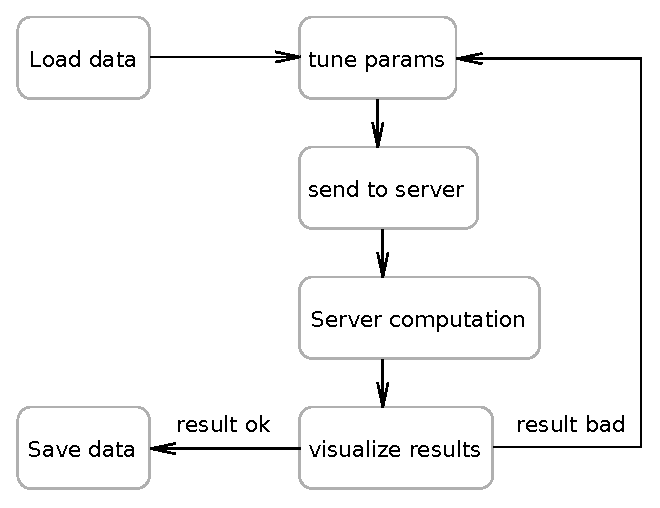
\includegraphics[width=14cm]{data/computationProcess.eps}
    \caption[RemoteCellLevelSet application computation process]{Client acts like GUI for the server side that performs actual computation}
    \label{fg:computationProcess}
\end{figure}

\par
There was some neccessary goals for incorporate 'pok' into Medv4D framework:
\begin{enumerate}
  \item{ITK integration}
  \par
  This is performed by wrapper Medv4D filter that is connected into Medv4D pipeline. Within this filter are two ITK images that serves as input and output for inner ITK pipeline. Actual data of this ITK images point to data of containing Medv4D wrapper filter (see Figure \ref{fg:ITKWrapping} for details).

  \item{Remote computing infrastructure}
  \par
  Infrastructure for sending commands to server along with data or parameter values as well recieving response messages along with resulting data had to be implemented into Medv4D. It lead into designing whole new library of Medv4D called remote computing. On client side it is representing by a remote filter that encapsulate whole infrastructure necessary for sending part of pipeline that the filter represents to server as well as result handling. Server side had to be designed completely as a whole.
\end{enumerate}

\begin{figure}
    \centering
    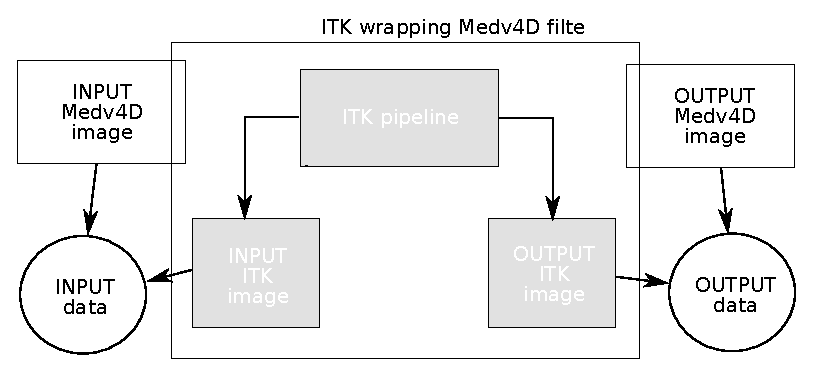
\includegraphics[width=12cm]{data/ITKFilter.eps}
    \caption[ITK wrapper Medv4D filter]{Basic elements are the two ITK images whose data are actually Medv4D images' data}
    \label{fg:ITKWrapping}
\end{figure}

\subsection{Client part of remote computing}



\subsection{Server part of remote computing}